\documentclass[10pt,a4paper]{jlreq}
%\documentclass[10pt,a4paper]{ltjsarticle}

\usepackage{graphicx}
\usepackage[pdfencoding=auto]{hyperref}
\usepackage{amsmath,amssymb}
\usepackage{bm}
\usepackage{booktabs}
%\usepackage{subfig}
\usepackage{pifont}
\usepackage{url}
\usepackage{cite}
\usepackage{ulem}
\usepackage{siunitx}
\usepackage{float}
\usepackage{tcolorbox}
\tcbuselibrary{breakable}
\usepackage{cancel}
\usepackage{color}
\renewcommand{\CancelColor}{\color{red}}

\usepackage{tikz}
\usetikzlibrary{shadows}
\usetikzlibrary{calc}
%\usepackage{circuitikz}

\usepackage{luatexja-fontspec}
%\setmainfont{TimesNewRoman}
%\setsansfont{Arial}
%\defaultjfontfeatures{Scale=1.0}
%\setmainjfont[BoldFont=IPAexGothic]{IPAexMincho}
%\setsansjfont{IPAexGothic}
\renewcommand{\figurename}{Fig.~}
\renewcommand{\tablename}{Table~}

\hypersetup{
  colorlinks=false, % リンクに色をつけない設定
  %bookmarks=true, % 以下ブックマークに関する設定
  bookmarksnumbered=true,
  pdfborder={0 0 0},
  bookmarkstype=toc
}

\begin{document}
\title{シンクロトロン振動のいろは}
\author{吉本伸一}
\maketitle
\tableofcontents
\clearpage

\section{はじめに}
シンクロトロンでは、ビームに対して横方向(水平,垂直方向)には四極磁石による収束力が働き、縦方向(進行方向)には高周波加速による収束力が働いている。これらの収束力によって、ビームはその平衡点の周りを振動しながら周回する。この横方向の振動をベータトロン振動と呼び、縦方向の振動をシンクロトロン振動と呼ぶ。ここでは、主に縦方向の運動について考えていくことにする。

\section{シンクロトロンの基礎の基礎}
シンクロトロンは、荷電粒子が偏向電磁石によって曲げられ、高周波加速空洞によって加速される円形加速器である (Fig.~\ref{synchrotron}) 。線形加速器とは異なり、粒子は閉軌道を周回し、加速空洞で繰り返し加速される。
%
\begin{figure}[hbt]
  \begin{center}
    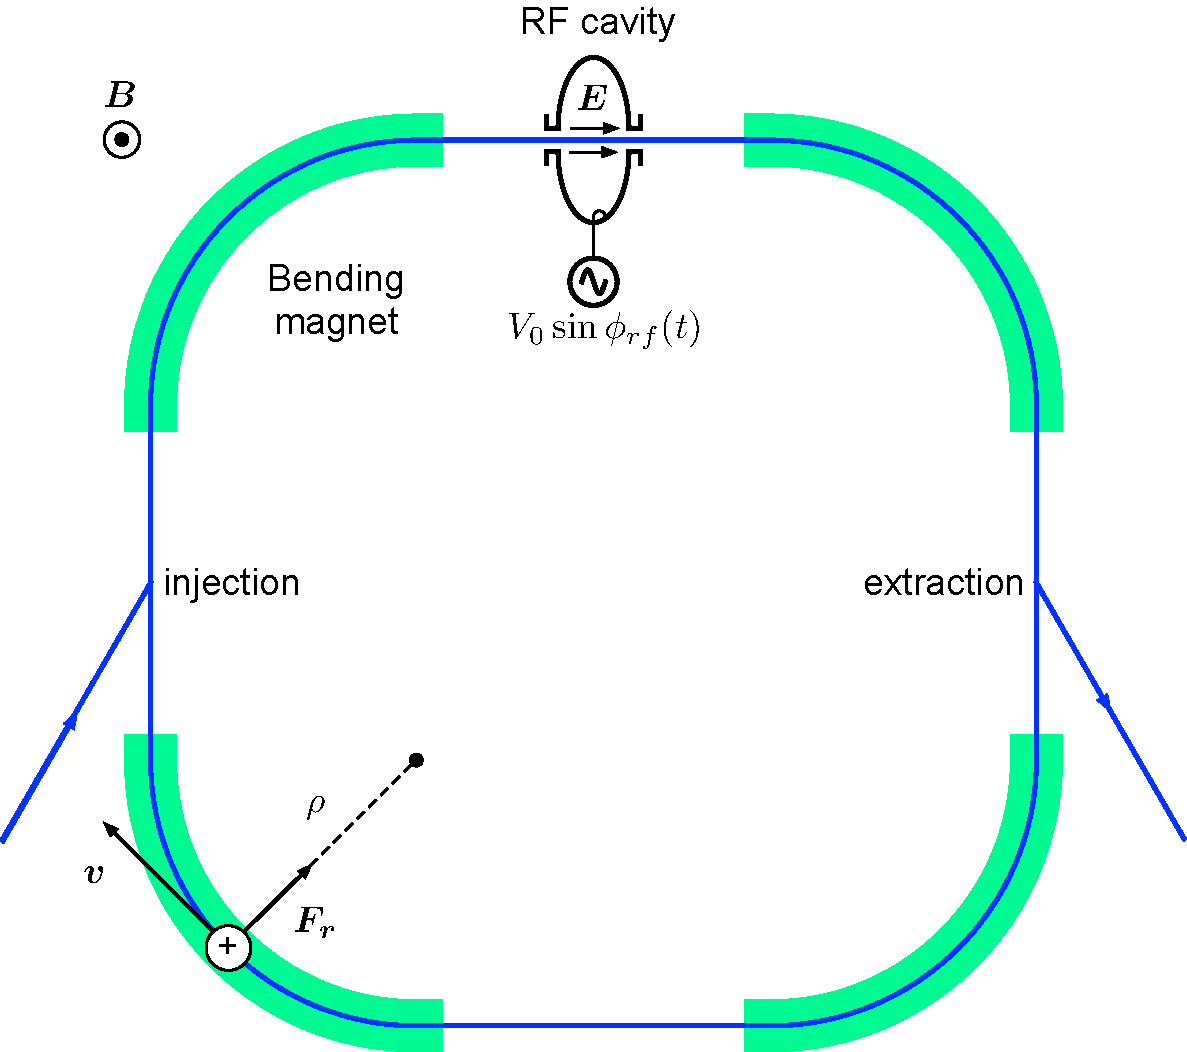
\includegraphics[width=12cm,clip]{figs/synchrotron.pdf}
    \caption{シンクロトロンの概略図.}
   \label{synchrotron}
  \end{center}
\end{figure}

粒子の運動方程式は、
%
\begin{equation}
  \frac{d\bm{p}}{dt} = e (\bm{E} + \bm{v}\times \bm{B})
\end{equation}
%
となるが、動径方向の運動を考えると
%
\begin{equation}
  \frac{m v^2}{\rho} = |\bm{F_r}| = e v B
\end{equation}
%
したがって、粒子の運動量と磁場の間には次の関係が成り立つ。
%
\begin{equation}
  p = mv = e \rho B
  \label{momentum_B}
\end{equation}
%
粒子の運動量は加速空洞で加速される毎に増加するので、曲率半径と周回軌道を一定に保つためには、(\ref{momentum_B}) より、偏向電磁石の磁場$B$は運動量に比例して増加しなければならない。また、回転周波数$f_{rev}$も運動量と共に増加するので、粒子と加速電圧の同期を維持するために加速周波数$f_{RF}$も追随する必要がある。

\section{同期粒子}

\begin{figure}[hbt]
  \begin{center}
    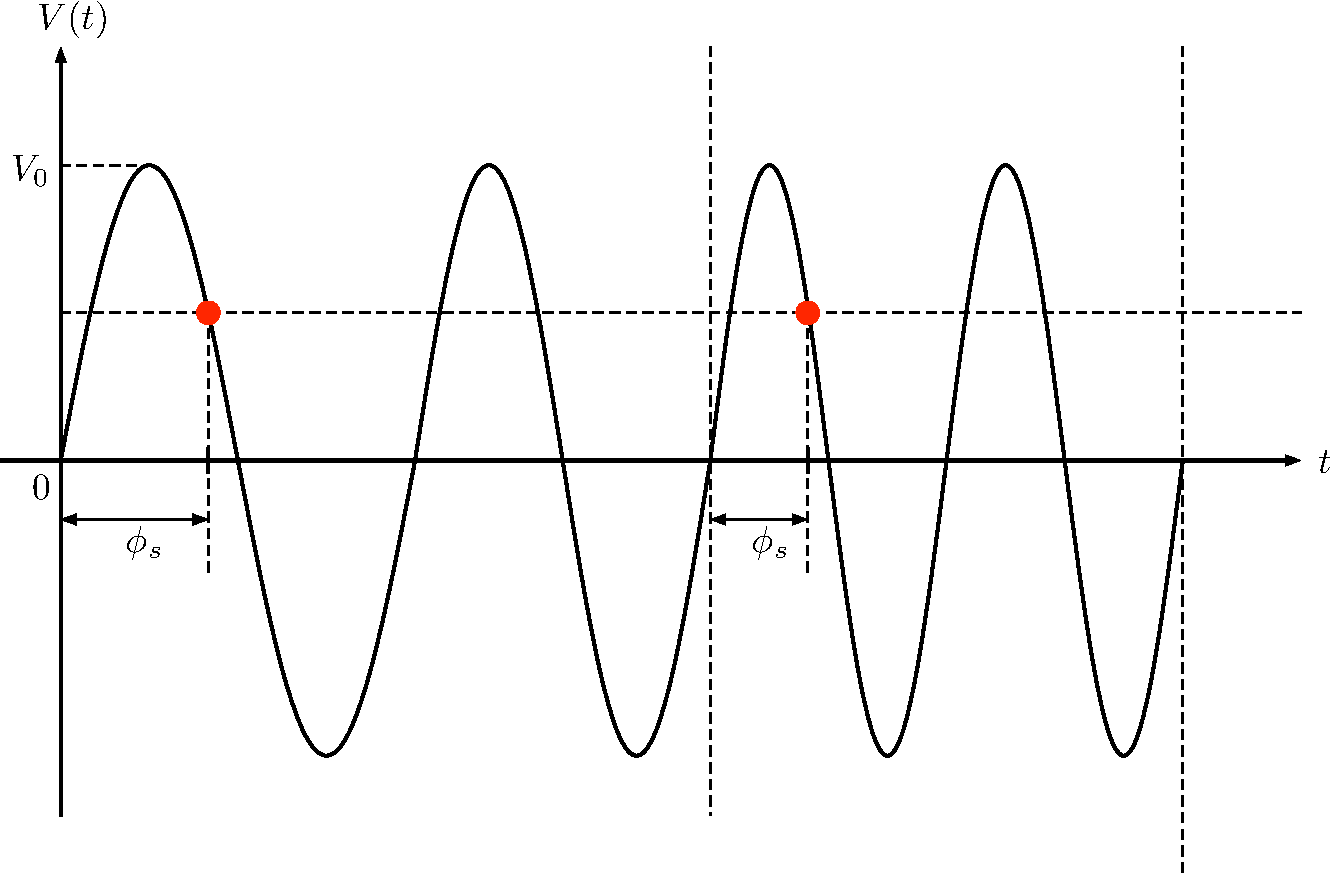
\includegraphics[width=15cm,clip]{figs/synchronous.pdf}
    \caption{同期粒子と空洞電圧の関係 ($h=2$ の場合).}
    \label{synchronous}
  \end{center}
\end{figure}

基準軌道を周回し、毎周同じ位相で加速空洞を通過する粒子を同期粒子 (synchronous particle) と呼び、その位相$\phi_s$のことを同期位相 (synchronous phase) と言う。同期粒子であるためには、周回周波数$f_{rev}$と空洞の加速周波数$f_{RF}$の間に、ある整数$h$を用いて、
%
\begin{equation}
  f_{RF} = h f_{rev}
  \label{harmonic}
\end{equation}
%
という関係が必要である。この整数$h$のことをharmonic numberと言い、加速周波数$f_{RF}$で加速できる最大の粒子数になる。この時、空洞の加速電圧は
%
\begin{equation}
  \begin{split}
    V_c (t) = V_0 \sin \phi_{RF}(t) \\
    \phi_{RF}(t) = \int_0^t \omega_{RF}(t) dt
  \end{split}
\end{equation}
%
となる。Fig.~\ref{synchronous}は、$h=2$の時の空洞電圧と同期粒子の関係を表してる。

\vspace{\baselineskip}

\begin{tcolorbox}[title=\textgt{SuperKEKBにおける$f_{RF}$, $f_{0}$, $h$}の関係]
  SuperKEKBの主リングでは、電子と陽電子はほぼ光速$c$で回っており、周長$C_0$は$\SI{3016.315}{\meter}$なので周回周波数$f_{rev}$は
  %
  \begin{equation}
    f_{rev} = \frac{1}{T_{rev}}=\frac{c}{C_0}=\frac{\SI{2.99792458e8}{\meter / \second}}{\SI{3016.315}{\meter}}=\SI{99.39}{\kilo\hertz} \notag
  \end{equation}
  %
  一方、加速周波数$f_{RF}$は$\SI{508.887}{\mega\hertz}$なので
  %
  \begin{equation}
      f_{RF} = 5120 \times f_{rev} \notag
  \end{equation}
  となり、確かに(\ref{harmonic})を満たしている。
\end{tcolorbox}

\section{Dispersion effects in a synchrotron}
シンクロトロンでは、偏向電磁石によって分散 (dispersion) が発生する為、粒子の横方向と縦方向の運動が結合する。この結合が、リングを周回する粒子の縦方向の運動において重要な役割を演じる。今、同期粒子の運動量を$p_s$とし、運動量偏差 (momentum deviation) を
%
\begin{equation}
  \delta_p = \frac{p-p_s}{p_s}=\frac{\Delta p}{p_s}
\end{equation}
%
\begin{figure}[hbt]
  \begin{center}
    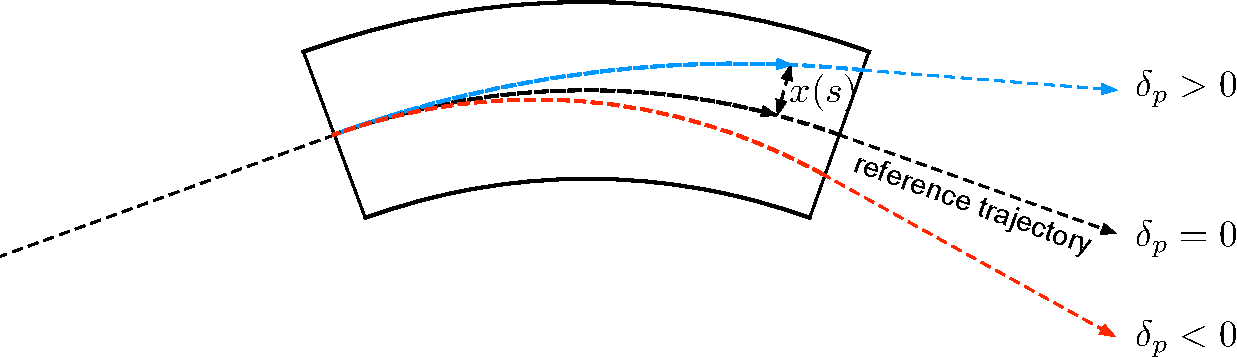
\includegraphics[width=15cm,clip]{figs/dispersion.pdf}
    \caption{偏光電磁石による基準軌道からのずれ (dispersion).}
    \label{dispersion}
  \end{center}
\end{figure}
%
とした時、$\delta_p = 0$でない粒子が偏光磁石を通過する場合を考える(Fig.~\ref{dispersion})。$\delta_p >0$ の場合、運動量の大きな粒子ほど偏光磁石で曲げられにくく、粒子は基準軌道より外側の軌道を通ることになる。一方、$\delta_p<0$の場合、粒子は同期粒子より曲げられ基準軌道より内側の軌道を通ることになる。この軌道のずれ$x(s)$は分散関数 (dispersion function) $D_x(s)$を用いて、
%
\begin{equation}
  x(s) = D_x(s)\frac{\Delta p}{p_s} = D_x(s)\delta_p 
\end{equation}
%
と表される。今、基準軌道の曲率半径を$\rho$とすると$ds = \rho d\theta$より (Fig.~\ref{momentum_compaction})、
%
\begin{equation}
  dC = (\rho + x) d\theta = (\rho + x) \frac{ds}{\rho}
\end{equation}
%
\begin{figure}[hbt]
  \begin{center}
    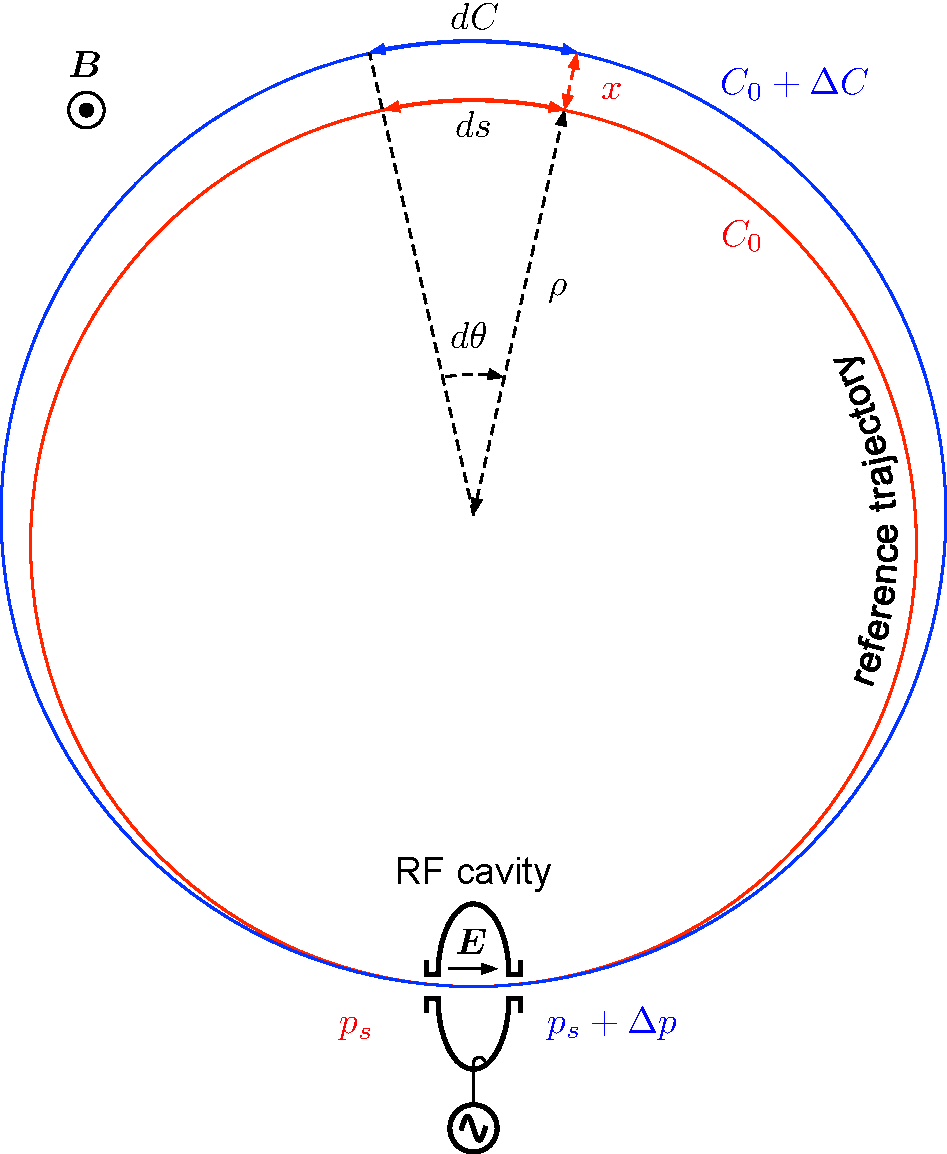
\includegraphics[width=10cm,clip]{figs/momentum_compaction.pdf}
    \caption{Momentum compaction factor.}
    \label{momentum_compaction}
  \end{center}
\end{figure}
%
したがって、この粒子の軌道長 $C$ は、
%
\begin{align}
  C &= \oint (\rho + x)\frac{ds}{\rho} = \int_0^{C_0} ds + \int_0^{C_0}\frac{x}{\rho} ds \notag \\
  &= C_0 + \delta_p \int_0^{C_0}\frac{D_x(s)}{\rho} ds
\end{align}
%
ここで運動量圧縮率 (momentum compaction factor) $\alpha_p$ を
%
\begin{equation}
  \alpha_p \equiv \frac{1}{C_0} \oint \frac{D_x(s)}{\rho} ds
\end{equation}
%
と定義すると、軌道長の差 $\Delta C = C-C_0$ は、
%
\begin{equation}
  \frac{\Delta C}{C_0}=\alpha_p\frac{\Delta p}{p_s}=\alpha_p\delta_p
  \label{delta_C}
\end{equation}
%
となり$\alpha_p$は運動量の変化による相対的な軌道長の変化を表していることになる。

\section{トランジション・エネルギー}
加速空洞で加速された粒子は運動量が増加するため、先ほど見たように軌道長の増加と共に、速度も増加する。今、同期粒子の速度を$v_s$とし、同期粒子のローレンツ因子を
%
\begin{equation}
  \gamma_s = \frac{1}{\sqrt{1 - \beta_s^2}}, \quad \beta_s = \frac{v_s}{c}
\end{equation}
%
とすると、(\ref{dv_dp}) より、運動量の変化と速度の変化の間に以下の関係が成り立つ。
%
\begin{equation}
  \frac{\Delta v}{v_s}=\frac{1}{\gamma_s^2}\frac{\Delta p}{p_s}
  \label{delta_v}
\end{equation}
%
このように運動量の変化$\Delta p$によって、速度$\Delta v$と軌道長$\Delta C$が変化するが、それによって回転周期$T$は同期粒子の周期$T_{rev}=C_0/v_s$とすると、
%
\begin{equation}
  T = T_{rev} + \Delta T = \frac{C_0 + \Delta C}{v_s + \Delta v} \notag
\end{equation}
%
と変化する。分母を払って整理すると、(二次の微小量は無視する)
%
\begin{align}
  & (T_{rev} + \Delta T)(v_s + \Delta v) = C_0 + \Delta C \notag \\
  \Longleftrightarrow\quad & \underset{C_0}{\uwave{\cancel{v_s T_{rev}}}} + \Delta v T_{rev} + v_s \Delta T +
  \underset{0}{\uwave{\cancel{\Delta v \Delta T}}}
  = \cancel{C_0} + \Delta C \notag \\
  \Longleftrightarrow\quad & v_s \Delta T = \Delta C- \Delta v T_{rev} \notag \\
  \Longleftrightarrow\quad & \frac{\Delta T}{T_{rev}} = \frac{\Delta C_0}{\underset{C_0}{\uwave{v_s T_{rev}}}} - \frac{\Delta v}{v_s} \notag
\end{align}
%
したがって、$\Delta T$, $\Delta C$, $\Delta v$の関係は以下のようになる。
%
\begin{equation}
  \frac{\Delta T}{T_{rev}} = \frac{\Delta C}{C_0} - \frac{\Delta v}{v_s}
  \label{delta_T}
\end{equation}
%
(\ref{delta_T}) に (\ref{delta_C}) と (\ref{delta_v})を代入すると、
%
\begin{equation}
  \frac{\Delta T}{T_{rev}} = \left(\alpha_p - \frac{1}{\gamma_s^2}\right)\frac{\Delta p}{p_s} = \eta_p \delta_p
  \label{deltat_eta_deltap}
\end{equation}
%
ただし、
%
\begin{equation}
  \eta_p \equiv \alpha_p - \frac{1}{\gamma_s^2} = \frac{1}{\gamma_t^2} - \frac{1}{\gamma_s^2}
  \label{alppha_slip}
\end{equation}
%
はphase slip factorと言い、運動量の変化による相対的な回転周期$T$の変化率を表している。
%
運動量圧縮率が正の場合 ($\alpha_p>0$) を考える。このとき、粒子の運動量を増加させると経路長が増加する。 しかし、粒子の運動量がまだ低く、光度よりも十分遅い場合、粒子の運動量の増加による速度の増加は、運動量の増加による経路長の増加を越えることがあり得る。その結果、粒子の回転周期は短くなる ($\eta_p < 0$)。
一方、粒子の運動量が十分高く超相対論的粒子の場合、粒子の速度は既に光速に十分近く、運動量の増加による速度の増加は極僅かである。この場合、経路長の増加が速度の増加を上回り、粒子の回転周期は長くなる ($\eta_p>0$) 。$\eta_p = 0$の時、つまり
%
\begin{equation}
  \gamma_t = \frac{1}{\sqrt{\alpha_p}}
\end{equation}
%
では回転周期は運動量に依存しない。この$\gamma_t$をトランジション・エネルギー (transition energy) と言う。

\vspace{\baselineskip}

\begin{tcolorbox}[title=\textgt{SuperKEKB LERのtransition energy}]
  SuperKEKBの陽電子リングLERの運動量圧縮率は$\alpha_p = 3.2 \times 10^{-4}$なので、
  %
  \begin{equation}
    \gamma_t = \frac{1}{\sqrt{\alpha_p}}= \frac{1}{\sqrt{3.2 \times 10^{-4}}} = 55.9 \notag
  \end{equation}
  %
  陽電子の静止質量は$E_0 = \SI{0.5109989461}{\mega\electronvolt}$だから
  \begin{equation}
    E = \gamma_t E_0 = \SI{28.6}{\mega\electronvolt} \notag
  \end{equation}
  %
  となり、入射器からの入射エネルギー$\SI{4}{\giga\electronvolt}$の方がtransition energyより十分高い。
\end{tcolorbox}

\section{位相安定性の原理}

\begin{figure}[hbt]
  \begin{center}
    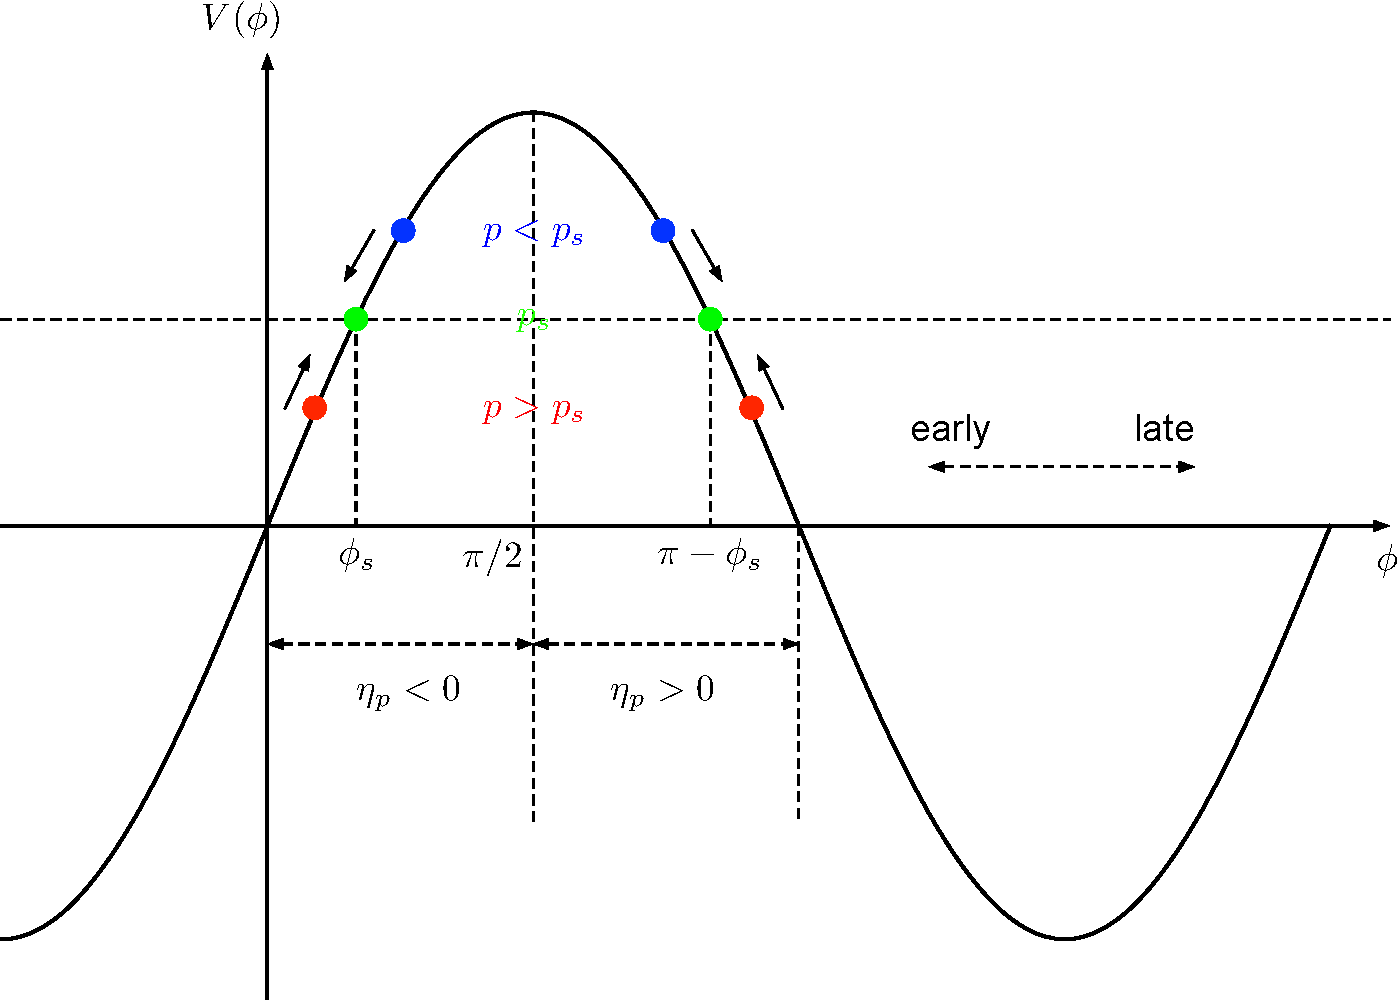
\includegraphics[width=15cm,clip]{figs/phase_stability.pdf}
    \caption{空洞電圧と同期粒子 $(p_s)$, より高い運動量を持つ粒子 $(p>p_s)$, より低い運動量 $(p<p_s)$ を持つ粒子の位相関係.}
    \label{phase_stability}
  \end{center}
\end{figure}

ビームの中には多くの粒子があり、色々な運動量を持つ粒子で構成されている。同期粒子と異なる運動量を持つ粒子が加速空洞を通過する時、どのように加速されるかについて考えてみる (Fig.~\ref{phase_stability}) 。

$\eta_p < 0$ の時、同期粒子より大きい運動量を持つ粒子 $(p>p_s$) は、同期粒子より回転周期が短いので、同期粒子より早く加速空洞に到着する。したがって、同期位相$\phi_s$を$0<\phi_s<\pi/2$に選べば、より大きい運動量を持つ粒子は、同期粒子より少ないエネルギーを加速空洞から得ることになる。同様に、同期粒子より小さな運動量を持つ粒子 $(p<p_s)$ は、同期粒子より遅く加速空洞に到達するので、同期粒子より多いエネルギーを加速空洞から得る。この過程を繰り返すことで、同期粒子の持つ運動量から外れた運動量を持つ粒子は同期粒子の周りを安定に運動することが分かる。$\eta_p > 0$ の時は、同期位相を$\pi/2<\phi_s<\pi$に選べば同様にこの運動は安定である。

\section{Difference Equations for Longitudinal Motion in a Synchrotron}
ここでは、粒子の周回毎の縦方向の運動について、これまでと同様にリングに加速空洞は一台だけ設置されている場合を考える。空洞電圧のゼロクロス点からの相対時間を$\tau$、相対位相を$\phi\pmod{2\pi}$とする (Fig.~\ref{coordinates})。今、$n+1$周回目の粒子の空洞への到着時間$\tau(n+1)$と$n$周回目の到着時間$\tau(n)$との差は、粒子の$n+1$周回目の回転周期$T(n+1)$と同期粒子の回転周期$T_{rev}(n+1)$との差に等しいので、
%
\begin{equation}
  \tau(n+1) - \tau(n) = T(n+1) -T_{rev}(n+1)
  \label{tau_T}
\end{equation}
%
\begin{figure}[hhbt]
  \begin{center}
    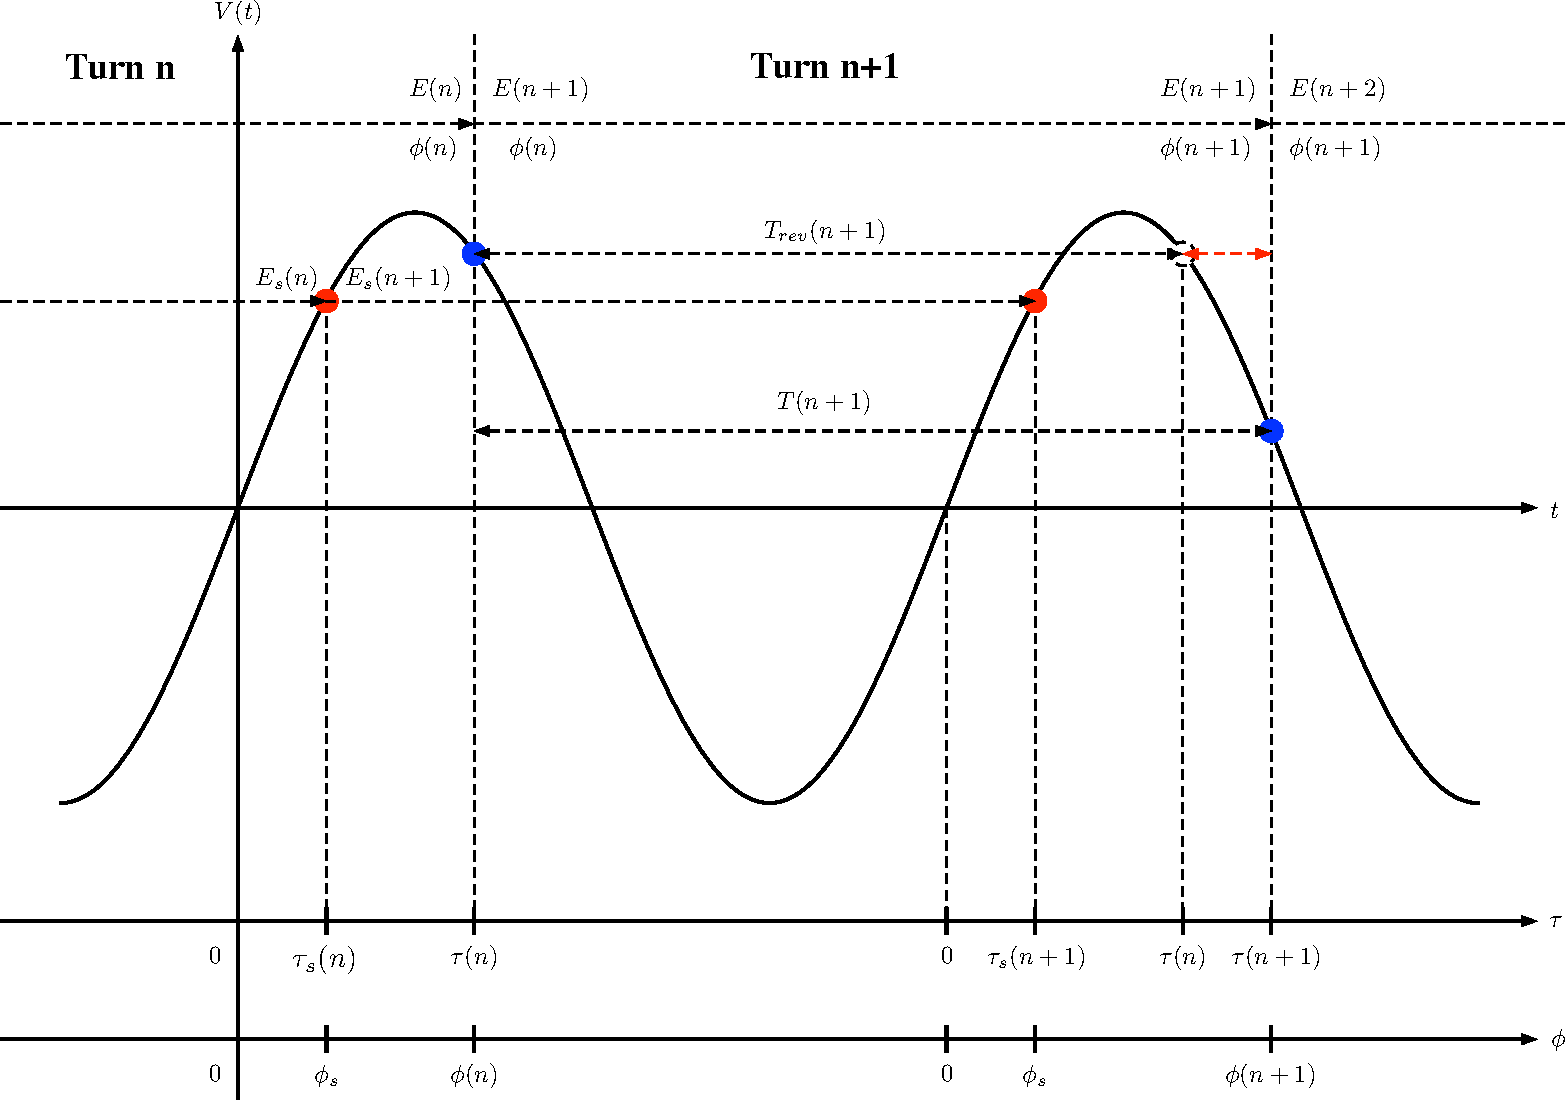
\includegraphics[width=15cm,clip]{figs/coordinates.pdf}
    \caption{空洞電圧と相対時間$\tau$, 相対位相$\phi$の関係 ($h=1$の場合).}
    \label{coordinates}
  \end{center}
\end{figure}
%
$\phi(n+1) = \omega_{RF}(n+1) \tau(n+1)$から、この関係を用いると、
%
\begin{align}
  \phi(n+1) &=\omega_{RF}(n+1)\{\tau(n) + T(n+1) -T_{rev}(n+1)\} \notag \\
    &= \frac{\omega_{RF}(n+1)}{\omega_{RF}(n)} \phi(n) + \omega_{RF}(n+1)\{T(n+1) -T_{rev}(n+1)\}  \notag
\end{align}
%
(\ref{deltat_eta_deltap})より
%
\begin{equation}
    \frac{T(n+1)-T_{rev}(n+1)}{T_{rev}(n+1)} = \eta \delta_p(n+1)
\end{equation}
%
を用いると、
%
\begin{align}
  \phi(n+1) &= \frac{\omega_{RF}(n+1)}{\omega_{RF}(n)}\phi(n) + \omega_{RF}(n+1)T_{rev}(n+1)\eta \delta_p(n+1) \notag \\
  &=\frac{\omega_{RF}(n+1)}{\omega_{RF}(n)}\phi(n) + 2\pi h \eta \delta_p(n+1)
\end{align}
%
ここで、
%
\begin{equation}
  \frac{\omega_{RF}(n+1)}{\omega_{RF}(n)} \approx 1
\end{equation}
%
という近似を行うと、位相に関して次の関係が成り立つ。
%
\begin{equation}
  \phi(n+1) = \phi(n) + 2\pi h \eta \delta_p(n+1)
\end{equation}

次に、$n+1$周回目の粒子のエネルギー$E(n+1)$は、$E(n)$に位相$\phi(n)$で空洞を通過する時に得られるエネルギーを足し合わせたものだから、
%
\begin{equation}
  E(n+1) = E(n) + e V \sin\phi (n)
\end{equation}
%
同期粒子に関しても同様に考えると、
%
\begin{equation}
  E_s(n+1) = E_s(n) + e V \sin\phi_s
\end{equation}
%
両辺の差を取り、$\Delta E = E - E_s$とすると、
%
\begin{equation}
  \Delta E(n+1) = \Delta E(n) + e V (\sin\phi(n) - \sin\phi_s)
\end{equation}
%
ここで、(\ref{dp_de})より、
%
\begin{equation}
  \delta_p = \frac{\Delta p}{p_s} = \frac{1}{\beta_s^2}\frac{\Delta E}{E_s}
  \label{delta_p}
\end{equation}
%
より、
%
\begin{equation}
  \Delta E(n+1) - \Delta E(n) = \beta^2 E_s \{\delta_p(n+1) - \delta_p(n)\}
\end{equation}
%
したがって、
%
\begin{equation}
  \delta_p(n+1) - \delta_p(n) = \frac{e V}{\beta_s^2 E_s}(\sin\phi(n) -\sin\phi_s)
\end{equation}
%

以上より、シンクロトロンの縦方向の運動について、周回毎の差分方程式は以下のようになる。
%
\begin{align}
  \begin{split}
     &\delta_p(n+1) = \delta_p(n) + \frac{e V}{\beta_s^2 E_s}(\sin\phi(n) -\sin\phi_s) \\
     &\phi(n+1) = \phi(n) + 2\pi h \eta \delta_p(n+1)
    \label{map}
  \end{split}
\end{align}
%
これらの式より、$(\phi(n),\,\delta_p(n))$の値を順次求めることで縦方向の運動を調べることができる (particle tracking simulation)。

\section{Differential Equations for Longitudinal Motion in a Synchrotron}
$\phi$と$\delta_p$のリング一周あたりの変化が十分小さい時、離散的な差分方程式である (\ref{map}) は、連続的な微分方程式に書き換えることができる。この場合、$\phi$と$\delta_p$のリング一周あたりの変化はそれぞれ、近似的に
%
\begin{equation}
  \frac{\delta_p(n+1)-\delta_p(n)}{T_{rev}(n+1)} \approx \frac{d\delta_p}{dt}=\dot{\delta_p},\quad 
  \frac{\phi(n+1)-\phi(n)}{T_{rev}(n+1)} \approx \frac{d\phi}{dt}= \dot{\phi}
\end{equation}
%
と書けるので、(\ref{map}) は
%
\begin{align}
    \begin{split}
      \dot{\delta_p} &= \frac{e V \omega_{rev}}{2\pi \beta_s^2 E_s}(\sin\phi - \sin\phi_s) \\
      \dot{\phi} &= h \omega_{rev} \eta \delta_p
    \end{split}
\end{align}
%
この二つの式をまとめると、
%
\begin{equation}
  \ddot{\phi} = \frac{e V h \eta \omega_{rev}^2}{2\pi\beta_s^2 E_s}(\sin\phi-\sin\phi_s)
  \label{ddot_phi}
\end{equation}
%
$\Delta\phi = \phi - \phi_s$が非常に小さい時、
%
\begin{equation}
  \sin\phi = \sin(\phi_s+\Delta\phi) \approx \sin\phi_s + \cos\phi_s \Delta\phi
\end{equation}
%
より (\ref{ddot_phi}) は
%
\begin{equation}
  \ddot{\Delta\phi} = \frac{e V h \eta \omega_{rev}^2}{2\pi \beta_s^2 E_s} \cos\phi_s \Delta\phi = - \omega_s^2 \Delta\phi
\end{equation}
%
となり、この運動は$\phi_s$の周りの単振動であることが分かる。また、この振動の振動数$\omega_s$は
%
\begin{equation}
  \omega_s = \sqrt{-\frac{e V h \eta \omega_{rev}^2 \cos\phi_s}{2\pi \beta_s^2 E_s}}
\end{equation}
%
となり、これをシンクロトロン振動数と呼ぶ。
%
\vspace{\baselineskip}

\begin{tcolorbox}[title=\textgt{SuperKEKBのシンクロトロン周波数}, breakable = true]
  SuperKEKB両リングのシンクロトロン振動に関係するパラメータは、

  \vspace{\baselineskip}

  \begin{center}
    \begin{tabular}{l|c|cc|c}
      & & LER   &   HER & units \\ \hline
      Beam Energy & $E_s$ & 4.000 & 7.007 & GeV  \\
      Momentum Compaction & $\alpha_p$ & $3.20\times 10^{-4}$& $4.55\times 10^{-4}$ & \\
      Total Cavity Voltage & $V_c$ & 9.4   &   15.0  &   MV \\
      Energy Loss/turn & $U_s$   & 1.76  &   2.43  & MeV \\
      RF frequency & $f_{RF}$ & \multicolumn{2}{c|}{508.887} & MHz \\
      Harmonic number & $h$       &   \multicolumn{2}{c|}{5120}  &
    \end{tabular}
  \end{center}
  
  \vspace{\baselineskip}

  同期位相$\phi_s$は$U_s = e V_c \sin \phi_s$から求まり、LERの場合
  %
  \begin{equation}
    \sin \phi_s = \frac{U_s}{e V_c} = \frac{\SI{1.76}{\mega\electronvolt}}{\SI{9.4}{\mega\electronvolt}} \notag
  \end{equation}
  %
  陽電子の静止質量$E_0 = \SI{0.5109989461}{\mega\electronvolt}$を使うと、$\gamma$, $\eta$, $\beta_s$は
  \begin{equation}
    \gamma = \frac{E_s}{E_0}\,, \quad \eta = \alpha_p - \frac{1}{\gamma^2}\,, \quad \beta_s = \sqrt{1-\frac{1}{\gamma^2}} \notag
  \end{equation}
  %
  から求まる。また、周回周波数$f_{rev}$は
  %
  \begin{equation}
    f_{rev} = \frac{f_{RF}}{h} = \frac{\SI{508.887}{\mega\hertz}}{5120} = \SI{99.39}{\kilo\hertz} \notag
  \end{equation}
  %
  以上より、LERのシンクロトロン周波数は
  %
  \begin{equation}
    f_s = \sqrt{\frac{e V_c h \eta f_{rev}^2 \cos \phi_s}{2\pi \beta_s E_s}} = \SI{2.438}{\kilo\hertz}\notag
  \end{equation}
  %
  また、LERのシンクロトロン・チューン$\nu_s$は
  %
  \begin{equation}
    \nu_s = \frac{f_s}{f_{rev}} = 0.0245 \notag
  \end{equation}
  %
  となり、約41周で1回振動することになる。同様にしてHERの方も求めると
  %
  \begin{equation}
    f_s = \SI{2.782}{\kilo\hertz}, \, \nu_s = 0.0280 \notag
  \end{equation}
  %
  となり、約36周で1回振動することになる。何も非常にゆっくりとした振動である(ベータトロン振動と比べてみる)。
\end{tcolorbox}

\clearpage

\appendix
\renewcommand{\theequation}{\Alph{section}.\arabic{equation} }
\setcounter{equation}{0}

\section{相対論のおさらい}
静止エネルギー$E_0$, 静止質量$m_0$, 光速$c$, 運動エネルギー$E_k$, 全エネルギー$E$として、
%
\begin{equation}
  \begin{split}
    E_0 = m_0 c^2 ,\quad E = E_0 + E_k = mc^2\\
    \beta =\frac{v}{c}, \quad \gamma = \frac{E}{E_0}=\frac{m}{m_0}=\frac{1}{\sqrt{1-\beta^2}}
    \label{rest_energy}
  \end{split}
\end{equation}
%
また、運動量$p$とエネルギー$E$は
\begin{align}
  p &= mv = \gamma m_0 v = \gamma m_0 \beta c \label{momentum} \\
  E &= \gamma E_0 = \gamma m_0 c^2 \label{energy}
\end{align}
%
これより、
%
\begin{equation}
  \frac{p}{E} = \frac{\gamma m_0 \beta c}{\gamma m_0 c^2} = \frac{\beta}{c}
\end{equation}
%
(\ref{rest_energy})より、
%
\begin{equation}
  \beta = \sqrt{1-\frac{1}{\left(1+ E_k/E_0\right)^2}}
\end{equation}
%
電子の静止質量$E_0 = \SI{0.511}{\mega\electronvolt}$, 陽子の静止質量$E_0 = \SI{938}{\mega\electronvolt}$であるので、運動エネルギーとそれぞれの粒子の速度の関係をプロットすると、

\begin{figure}[hhbt]
  \begin{center}
    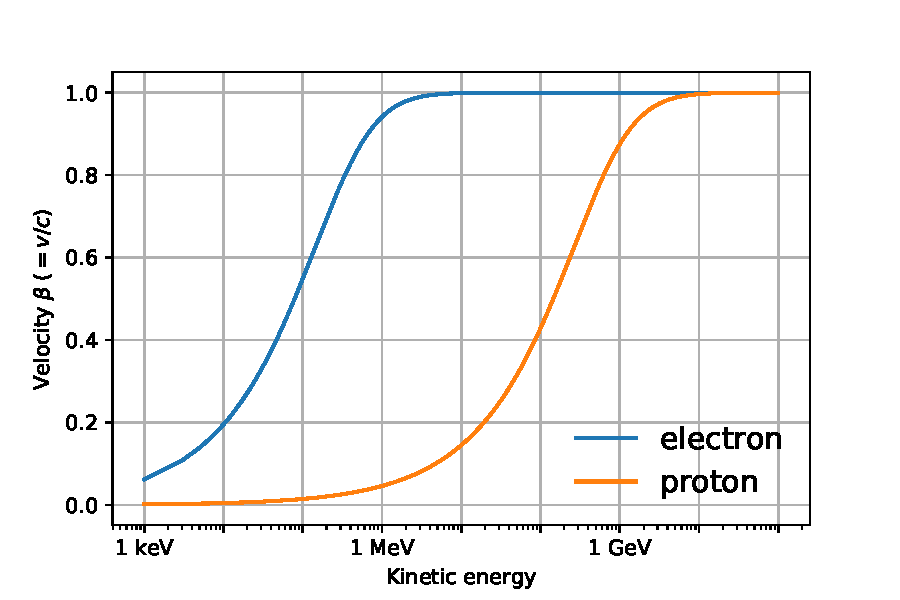
\includegraphics[width=12cm,clip]{figs/velocity.pdf}
    \caption{電子と陽子の運動エネルギーと速度の関係.}
    \label{velocity}
  \end{center}
\end{figure}

このグラフより、電子の速度は十分低いエネルギーでほぼ光速になっていることが分かる。
%
\paragraph{(\ref{delta_v}) の導出} \leavevmode\\

(\ref{momentum}) より、$p$を$v$で微分すると
%
\begin{equation}
  \frac{dp}{dv} = m_0\frac{d}{dv}(\gamma v)
  = m_0 \left(\gamma + v \frac{d\gamma}{dv}\right) \notag
\end{equation}
%
(\ref{rest_energy}) より、
%
\begin{align}
  \frac{d\gamma}{dv} & = \frac{1}{c}\frac{d\gamma}{d\beta}= \frac{1}{c}\frac{d}{d\beta}\left(\frac{1}{\sqrt{1-\beta^2}}\right) \notag \\
  & = \frac{1}{c} \beta \underset{\gamma^{-2}}{\uwave{(1-\beta^2)}}^{-\frac{3}{2}} = \frac{\beta \gamma^3}{c} \notag
\end{align}
%
これより、
\begin{align}
  \frac{dp}{dv} & = m_0 \left(\gamma + v \frac{\beta \gamma^3}{c}\right)
  = m_0 \gamma \underset{\gamma^2}{\uwave{(1 + \beta^2 \gamma^2)}}
  = \frac{\gamma^2 p}{v} \notag
\end{align}
%
したがって、
%
\begin{equation}
  \quad \frac{dv}{v} = \frac{1}{\gamma^2}\frac{dp}{p}
  \label{dv_dp}
\end{equation}
%
\paragraph{(\ref{delta_p})の導出}
%
\begin{align}
  p = mv = \gamma m_0 \beta c\,  , \quad E = \gamma E_0 = \gamma m_0 c^2 \notag
\end{align}
%
\begin{equation}
  \gamma \beta = \gamma \sqrt{1-\frac{1}{\gamma^2}} \notag = \sqrt{\gamma^2 -1} \notag
\end{equation}
%
\begin{align}
  \frac{dp}{dE} & = \frac{1}{c}\frac{d(\gamma \beta)}{d\gamma} = \frac{1}{c}\frac{d}{d\gamma}\sqrt{\gamma^2 -1} \notag \\
  & = \frac{\gamma}{c} \underset{\gamma^2\beta^2}{(\uwave{\gamma^2 -1}})^{-\frac{1}{2}} = \frac{1}{c\beta}
  = \frac{p}{\beta^2 E}\notag
\end{align}
%
したがって、
%
\begin{equation}
  \quad \frac{dp}{p} = \frac{1}{\beta^2}\frac{dE}{E}
  \label{dp_de}
\end{equation}

%
\begin{thebibliography}{9}
  \bibitem{oho}
  過去のOHOセミナーの教科書 \url{http://accwww2.kek.jp/oho/index.html}
\end{thebibliography}
%
\end{document}